%use the KomaScript styling on A4 paper
\documentclass[a4paper]{scrreprt}
%package for citing in Harvard style
\usepackage{natbib}
\bibliographystyle{agsm}
\usepackage[T1]{fontenc}
\usepackage[utf8]{inputenc}
\usepackage[none]{hyphenat}
\usepackage{graphicx}
\usepackage[hidelinks]{hyperref}
\usepackage{xurl}
\graphicspath{{"./figs"}}

%declare *bf* that is needed for natbib
\DeclareOldFontCommand{\bf}{\normalfont\bfseries}{\mathbf}
%set style of footnote numbering
\counterwithout{footnote}{chapter}

\begin{document}

\begin{titlepage}
\centering
{\large\textsc{Bachelor thesis}\par}
\vspace{8\baselineskip}
{\Huge The right-wing populism of the AfD party and its regional differences\par}
\vspace{2\baselineskip}
{\Large A quantitative analysis on populist antagonisms within the programmatic discourse\par}
\vspace{5\baselineskip}
{\large\textsc{submitted by\\[.5em]Dipl.-Math. Paul Keydel}\par}
\vspace{8\baselineskip}
{Freie Universität Berlin, April 2024\par}
\vfill
\raggedright
{\em 1st supervisor: Dr. Julia Reuschenbach\\}
{\em 2nd supervisor: Prof. Dr. Bruno Castanho Silva}
\end{titlepage}

\tableofcontents

%%%%%
% 1 %
%%%%%
\chapter{Introduction}
The aim of this thesis is to bla bla
%%%%%
% 2 %
%%%%%
\chapter{Populism as an ideology of democracy}
\section{What is an ideology?}
In order to understand the connection between populism and ideology, this section will outline a theoretical framework behind ideologies. There are, in general, several approaches within political theory to define or describe ideologies. For example, one might take policies into account and consider ideologies as attributions of them in a one-dimensional left-right spectrum. Such a policy-based approach can be useful for descriptive analysis of party alignment or voting behavior. \citep[p.~154]{lembcke:2014} But what is an ideology in itself?\par
The concept of attributing policies to ideologies suggests that ideologies are related to political issues and the way we think about politics. They originate from political thought, which is in turn expressed by a specific terminology and its meanings. With this, it opens up a discourse-analytical approach to ideologies that is particularly represented through the work of Michael Freeden. He claimed that the ``study of ideology becomes the study of the nature of political thought: its building blocks and the clusters of meaning with which it shapes the political worlds we populate''. \cite[p.~15]{freeden:2006} For him, the act of political thinking arises from real-world contexts and seeks interpretations of the political reality - within a specific terminological framework that is used to express and formulate these meaningful interpretations. Political thought is thus, too, a practice of building meanings and where individuals ``attempt [...] to impose specific senses on repositories of political meaning that are by their semantic nature multivalent and contestable''. \cite[p.~19]{freeden:2006} At this point, ideologies play a central role. They can structure the described process of political thought in the sense that ideologies both assign and fix specific meanings to political ideas or concepts. Freeden understands ideologies further as conceptual structures with which all political actors describe themselves, the relation between them and their relation to the surrounding world. Consequently, ideologies temporarily ``define our understanding of the political'' and they are thus dynamic, i.e. they change as political challenges of the society change. Within this dynamic alignment they also ``compete with alternative configurations over political support and over the central control of the political''. \cite[p.~14]{freeden:2006}\par
In his popular book {\em Ideologies and Political Theory} (1998) Freeden has developed a morphological approach to ideologies in order to explain and reconstruct the process of competition between conceptual elements and interpretations. His starting points are the already mentioned ``political concepts'' that stand for rather abstract ideas like ``liberty, justice, power and rights''. \cite[p.~54]{freeden:1998} These concepts are far from monolithic constructs, they rather consist of smaller {\em components} which can relate to each other and represent, through their specific configuration, the entire concept. Freeden distinguishes here between ``ineliminable'' and non-ineliminable\footnote{To be precise, non-ineliminable components are ``quasi-contingent''.} components. Ineliminable components are logically necessary, i.e. without any such components, it is impossible to derive a reasonable meaning. Thus, the set of all ineliminable components might be seen as the {\em core} of the concept, whereas non-ineliminable components ``cannot carry the concept on their own''. \cite[p.~62]{freeden:1998}\par
An analogous topology can be transferred to ideologies and conceptual structures, respectively. An ideology obtains and fixes meanings from multiple concepts and a single concept is not only determined by its components but also by its position within a greater ``idea-environment''. \cite[p.~67]{freeden:1998} In this manner, {\em adjacent concepts} emerge that, for example, share certain components and equally are part of the same ideology. Based on these considerations, Freeden postulates a three-level formation of ideologies: The most central concepts define the {\em core of the ideology}, supplemented by the concepts from the {\em adjacency} and the {\em periphery}. The example of liberalism illustrates this morphology:
\begin{quote}
    For instance, an examination of observed liberalisms might establish that liberty is situated within their core, that human rights, democracy, and equality are adjacent to liberty, and that nationalism is to be found on their periphery. \cite[p.~77]{freeden:1998}
\end{quote}
The advantage of Freeden’s morphology is that any configuration of concepts and its components is not isolated from other configurations. An ideology characterized by connections of concepts next to each other implies, inevitably, a certain ambiguity or indeterminacy, which again enables various narratives within the political struggle of consent and support. \cite[p.~155]{lembcke:2014}
\section{Populism and bridges between \guilsinglright the people\guilsinglleft\ and \guilsinglright the politics\guilsinglleft}
Populism is a widely used concept, not only in political science but also in media and public discourses. There is consequently more than one theoretical embedding of populism depending on populist aspects that will be analyzed. For example, following Chantal Mouffe and Ernesto Laclau, populism can be seen as a specific discourse practice to counteract neoliberal hegemony within a post-democratic society. Their (left-wing) populism is a positively connoted strategy to re-politize society by clarifying structures of oppression and exploitation. \citep{laclaumouffe:2001} However, when it comes to how left-wing and right-wing populism can be characterized in general, other theory buildings may be taken into account.\par
According to Cas Mudde, a more general theorizing of populism rests on ideational approaches; ``conceiving it as a discourse, an ideology, or a worldview''. \cite[p.~5]{mudde:2017} Although populism can take very different shapes in terms of political intentions or communication patterns, Mudde and Rovira Kaltwasser argue that populism at its heart is a ``kind of mental map through which individuals analyze and comprehend political reality''. \cite[p.~6]{mudde:2017} This common populist feature is directly linked to Freeden's conception on ideologies since a mental map constitutes a simpler picture on politics just as an ideology ``constitutes a significant sampling from the rich, but unmanageable and partly incompatible, variety of human thinking on politics''. \cite[p.~54]{freeden:1998} But, to distinguish populism from full-developed ideologies like liberalism, Mudde and Rovira Kaltwasser suggest a {\em restricted morphology}, i.e. populist concepts cannot offer comprehensive answers to any political issue. Instead, all patterns of populism mainly appeal to {\em the people} and are limited to a facile denunciation of {\em the elite}. Mudde finally defines populism as\par
\begin{quote}
    [...] a thin-centered ideology that considers society to be ultimately separated into two homogeneous and antagonistic camps, `the pure people' versus `the corrupt elite', and which argues that politics should be an expression of the volonté générale (general will) of the people. \cite[p.~6]{mudde:2017}
\end{quote}
Aside from this antagonistic relationship between the people and the elite and its possible consequences for populist discourses, one might ask the question of what can cause populist simplifications of reality. In the light of populist tendencies in democratic systems, this question becomes even more relevant, and referring to Margaret Canovan, there are in fact inner-democratic reasons for populism. She emphasizes an essential paradox that exists in democracies: The more people participate within the political arena, the more opinions and interests are part of the democratic discourse and the more difficult it is to conceptually overlook the arena, i.e. the ``most inclusive and accessible form of politics ever achieved is also the most opaque''. \cite[p.~25]{canovan:2002} In other words, the contradiction exists between the necessity of representing the people's concerns within the political process and the necessity of deriving clear interpretations of the people's political arena. It is hence a contradiction between ``bringing the people into politics'' and ``taking politics to the people'', and the responses to this are again populist attitudes. \cite[p.~26]{canovan:2002} Due to the complexity and variety of the political arena, people lean towards simplifications that is, the appeal to their `own' sovereignty against an unrepresentative elite that is supposed to be responsible for the lack of effective participation.\par
From a democratic point of view, the purpose of ideologies may be summed up in constructing bridges between {\em the people} and {\em politics}. They can offer a mental and intelligible map of the reality which becomes even more pressing within democracies, that are by their nature highly inclusive and complex. Populism, consequently, appears to be inherent in democracy - as the most vivid bridge. But paradoxically, according to Canovan, ideologies within democracies can always be misrepresentative regarding basic democratic principles. In this sense, the thin-centered populist ideology with its appeal to people’s sovereignty admittedly generates a simplification of the political arena but, on the other hand, creates a ``popular unity against multiplicity'' and a ``majority against minorities'', respectively. \cite[p.~26]{canovan:2002}. Such a contrariness, and in particular its discoursive construction is investigated in the following section.
\section{The role of antagonisms}
Roughly speaking, antagonisms are almost always the crucial element in constructing theoretical understandings of populism regardless of whether it is left-wing or right-wing. In Mouffe's and Laclau's conception of populism as a discoursive strategy, antagonisms are assumed to be the observable consequences of neoliberal hegemony. They need to be addressed by expressing all modes of oppression and exploitation equivalently in a linguistic chain associated with other social inequalities. Due to this chain of equivalent antagonisms, a discoursive momentum will be established to re-politicize society and repress the neoliberal hegemony. \cite[p.~135]{laclaumouffe:2001}\par
While the antagonistic configuration of left-wing populism is based on fights against poverty, privileged classes or ecological destruction, right-wing populism usually draws on other rivalries. But, as noted in the previous section, in all cases the use of antagonisms is required for constructing a specific dichotomy of {\em the people} and {\em the elite}. Following Mudde's definition, the concepts of the people and the elite are besides {\em the general will} the core concepts forming the populist ideology. As such they divide society into two distinct groups distinguishing between ``a homogeneous {\em good} and a homogeneous {\em evil}'' \cite[p.~7]{mudde:2017}. The concept of the people is thereby rather indeterminate: Who and what are the people? One answer was given by Laclau. According to him, the constitution of the people is a performative act. Laclau argues, similarly to Freeden, that meaning emerges with and through language and especially the construction of a collective identity like the people fundamentally depends on articulations between a logic of difference and a logic of equivalence. \cite[p.~x]{laclau:2005} Regarding the `good versus evil' dichotomy, he notes the importance of differential articulations within the production of meaning:
\begin{quote}
    This division [of society] presupposes the presence of some privileged signifiers which condense in themselves the signification of a whole antagonistic camp (the 'regime', the 'oligarchy', the 'dominant groups', and so on, for the enemy; the 'people', the 'nation', the 'silent majority', and so on, for the oppressed underdog - these signifiers acquire this articulating role according, obviously, to a contextual history). \cite[p.~87]{laclau:2005}
\end{quote}
From this perspective, it becomes obvious how antagonistic articulations meaningfully fill the political concept of the people that initially is just an ``empty signifier''. \cite[p.~72]{laclau:2005} Populism of all political colors hence requires several kinds of antagonisms to constitute the opposition between {\em us} and {\em them}. On the other side, several equivalent articulations are the discoursive basis for the {\em common cause}, i.e. they (re-)produce a ``shared identity'' between different groups and generate (political) affiliation. \cite[p.~9]{mudde:2017}\par
Putting all of this together, we can now identify the antagonistic nature of populism as an ideology of democracy. As the previous section pointed out, the people and the elite are supposed to be separated along the gap of power and the lack of effective participation. This specific dichotomy is not only articulated by attacks against selfish politicians, corrupt bureaucrats or democratic institutions in themselves, but also by attacks against those who are being identified as clients of the elite. That can involve asylum-seekers, migrants and certain minority groups and, typically, these groups are being negatively framed as ``beneficiaries of taxes paid by ordinary, hard-working people''. \cite[p.~32]{canovan:2002} This shows very plainly that racist discourses from the right-wing spectrum might affect the antagonistic articulation even more due to inherent practices of social othering. In general, since political concepts of right-wing movements or parties are related to multiple adjacent ideologies like nativism, authoritarianism or even Nazism, pure populist discourses can partly merge with others. Consequently, if one analyzes right-wing populism as we will do in the next chapter, the antagonistic constitution of {\em the people} should be considered multi-dimensionally.
%%%%%
% 3 %
%%%%%
\chapter{The AfD party and its right-wing populism}
\section{The party between populism and right-wing ideologies}
Within the political landscape in Germany, the AfD party ({\em Alternative für Deutschland}) became gradually successful and concerning current surveys they were the second political force in February 2024.\footnote{see \url{https://www.zdf.de/nachrichten/politik/politbarometer-afd-bsw-schuldenbremse-rechtsextremismus-ukraine-100.html}} The AfD party was founded in 2013 and can be seen as a so-called challenger party that claims to break with the established mainstream and the `old' tradition of catch-all parties. \citep{devries:2020} Nevertheless, the success of the AfD party is not merely a German phenomenon. Particularly the populist and right-wing challenger parties in Europe have been rising since the 1980s when one considers, for example, the French {\em Rassemblement national}, the Belgian {\em Vlaams Belang} or the Italian {\em Lega}. \cite[p.~30]{devries:2020} All these parties have a strong appeal to {\em the people} in common, and also they share other ideological key elements like xenophobia or nativism. That is because populism as a thin-centered ideology of democracy is a malleable conceptual structure and ``can easily be integrated into another more complex host ideology''. \cite[p.~19]{devries:2020}\par
In the book {\em The Far Right Today} Cas Mudde describes such adjacent ideologies that might serve as a host ideology. Following Mudde, the far right is first of all split into two groups, the ``extreme right'' and the ``populist radical right''. While the first group ideologically builds on historical fascism and fundamentally rejects democracy, the populist radical right supports democracy to some extent. Their ideological core consists of populism, nativism (a combination of both nationalism and xenophobia) and authoritarianism. \cite[p.~24]{mudde:2019} These three concepts generate a broader ideology according to which, first, society must be strictly ordered, second, citizenship is based on ethnicity and, third, mainstream parties keep the people from power. The consequent host ideology can additionally contain certain anti-religious elements such as antisemitism which has been part of right-wing ideologies since the twentieth century. \cite[p.~28]{mudde:2019} However, the ideological manifestation of far-right parties changes over time and a party's shift from a populist radical right ideology to extreme right might be fluent.\par
Especially the AfD party, in terms of its ideological basis, has been subject to change since its foundation. The party initially was a eurosceptic and economically liberal project but changed fast to a right-wing project during the migration crisis in 2014: According to their political communication on Facebook between 2013 and 2017, Arzheimer and Berning showed that the party ``has developed a clear focus on common populist radical right topics''. \cite[p.~3]{arzheimer:2019} But, even though the AfD party can be identified as a populist radical right project, extremist tendencies might have increased in the last years. The question arises of which ideologically induced prejudices they exactly express. In other words, who and what are the enemies?
\section{Ideological antagonisms at the level of the federal states}
The AfD party changed from Euroscepticism to (radical) right. Populist strategies against the government are common, also against immigration (Remigration).\\
Example of antagonistic speech: Telegram messages of the highest reaction rates!\\
Rating of the Verfassungsschutz concerning right-wing extremism is a potential East-West difference. The more extremistic the more concentration on ethnic aspects.\\
With this in mind, one might ask the question of whether the AfD party creates region-dependent populist narratives or a unique overall narrative related to right-wing antagonisms.
\begin{figure}
    \centering
    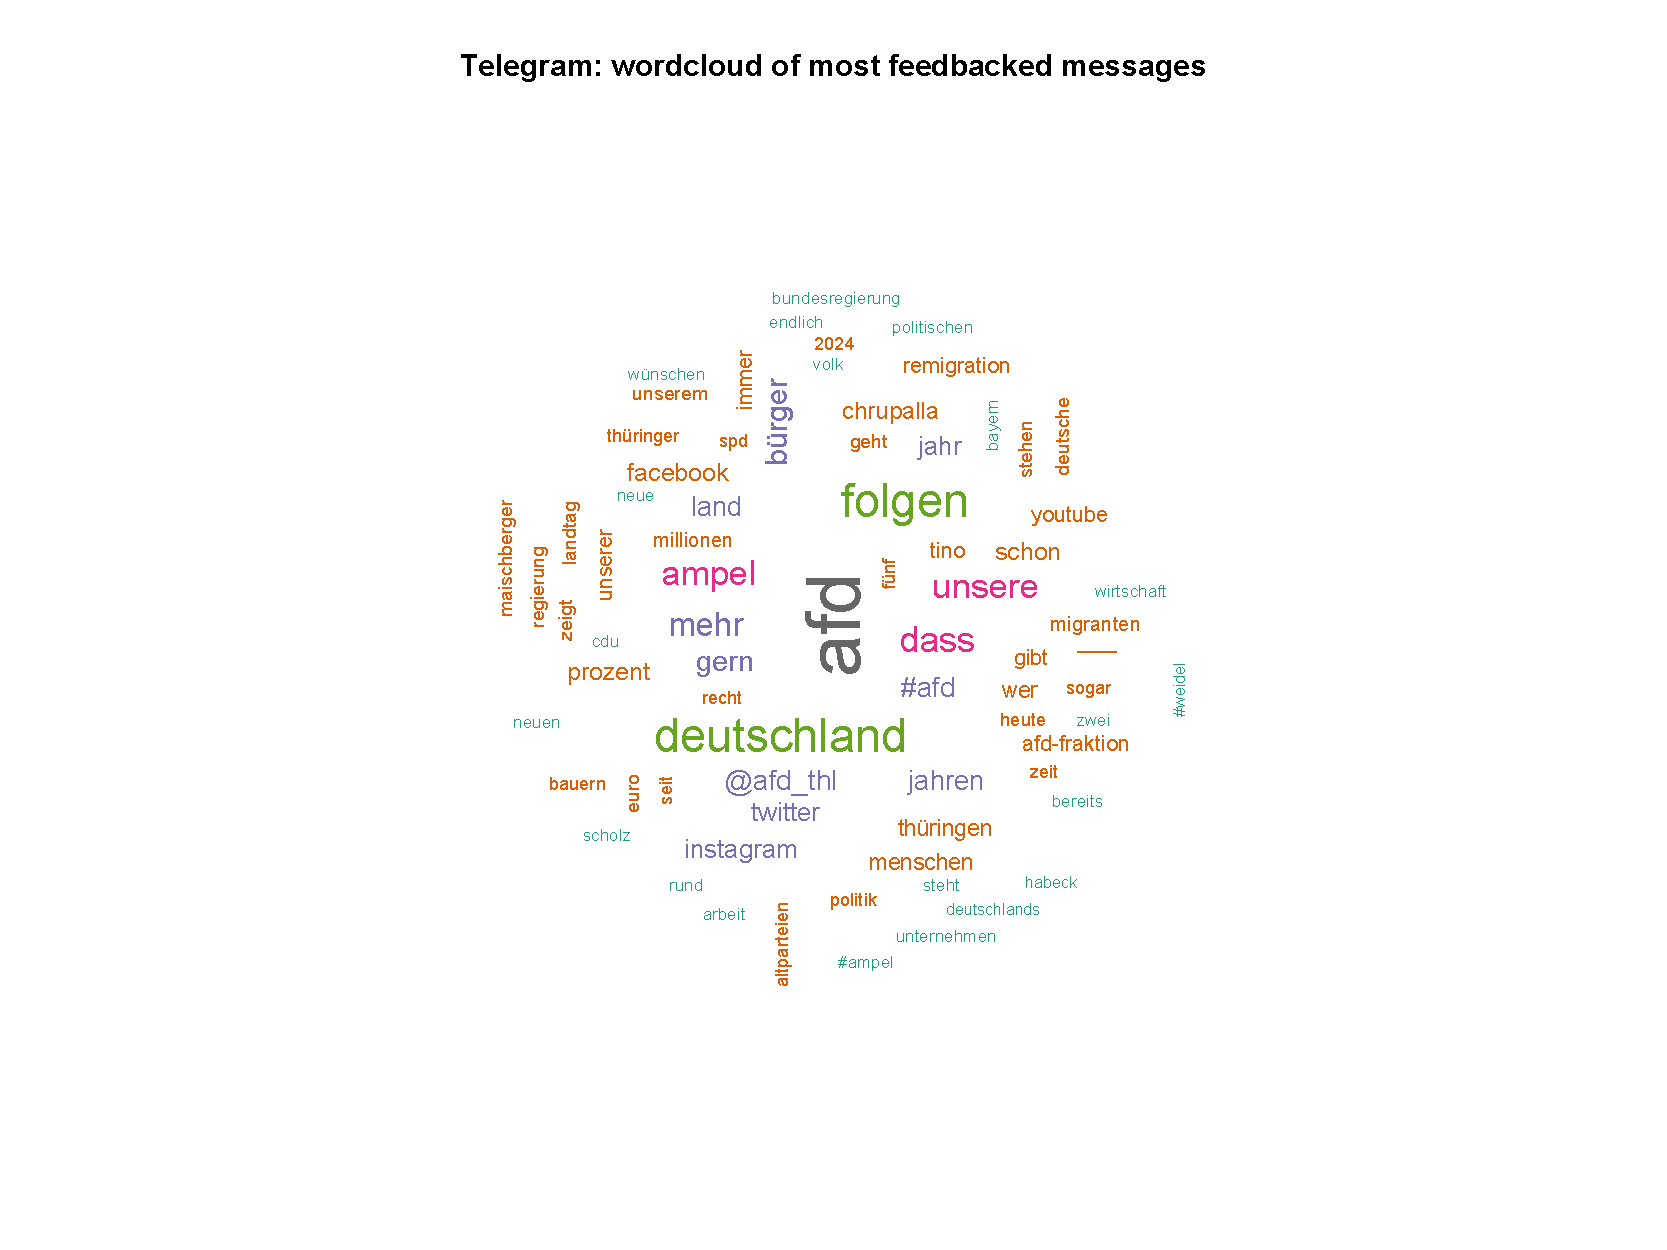
\includegraphics[width=0.9\textwidth]{telegram_wc_most_feedbacked.pdf}
    \caption{a nice plot}
\end{figure}
\section{Towards an analysis of the party manifestos}
Limit the analysis to the four subdicts from RPC. Why are these antagonisms relevant to the question in section 3.1.?\\
How can we achieve regional information on programmatic development? Manifestos are in this sense very helpful because they are created within a democratic process and therefore offer a deeper view inside the party.\\
Is there other current research that uses AfD manifestos? UK comparison, etc...\\
Which manifestos had specifically been chosen for this analysis, and why?
%%%%%
% 4 %
%%%%%
\chapter{An analysis of antagonisms within AfD manifestos}
\section{A dictionary-based approach with \em RPC-Lex}
What are dictionaries and how can they be used to measure populism?\\
What is the RPC-Lex and what is it used for? How was it constructed/collected?\\
Cite quanteda!
\begin{figure}
    \centering
    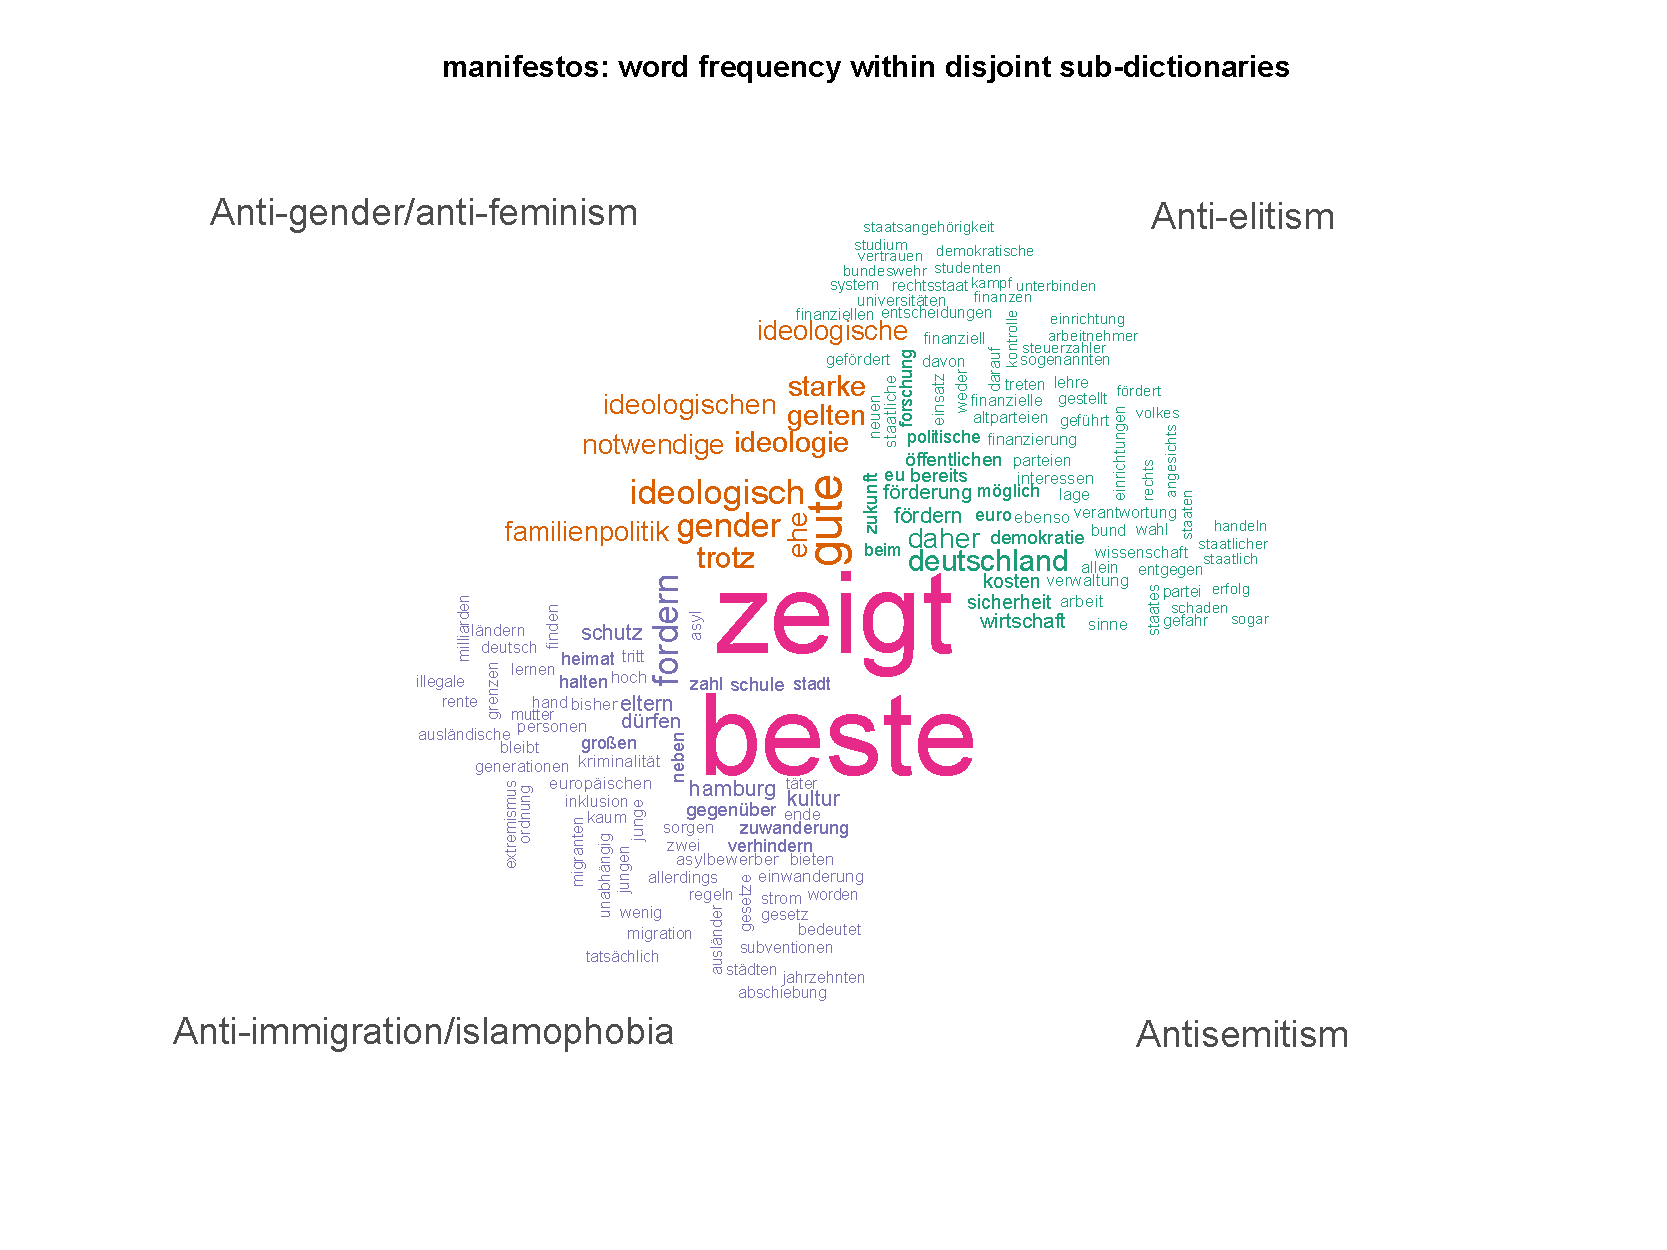
\includegraphics[width=0.9\textwidth]{manifestos_wordcloud_disjoint_subdicts.pdf}
    \caption{a nice plot}
\end{figure}
\section{Results for the last two state elections}
\begin{figure}
    \centering
    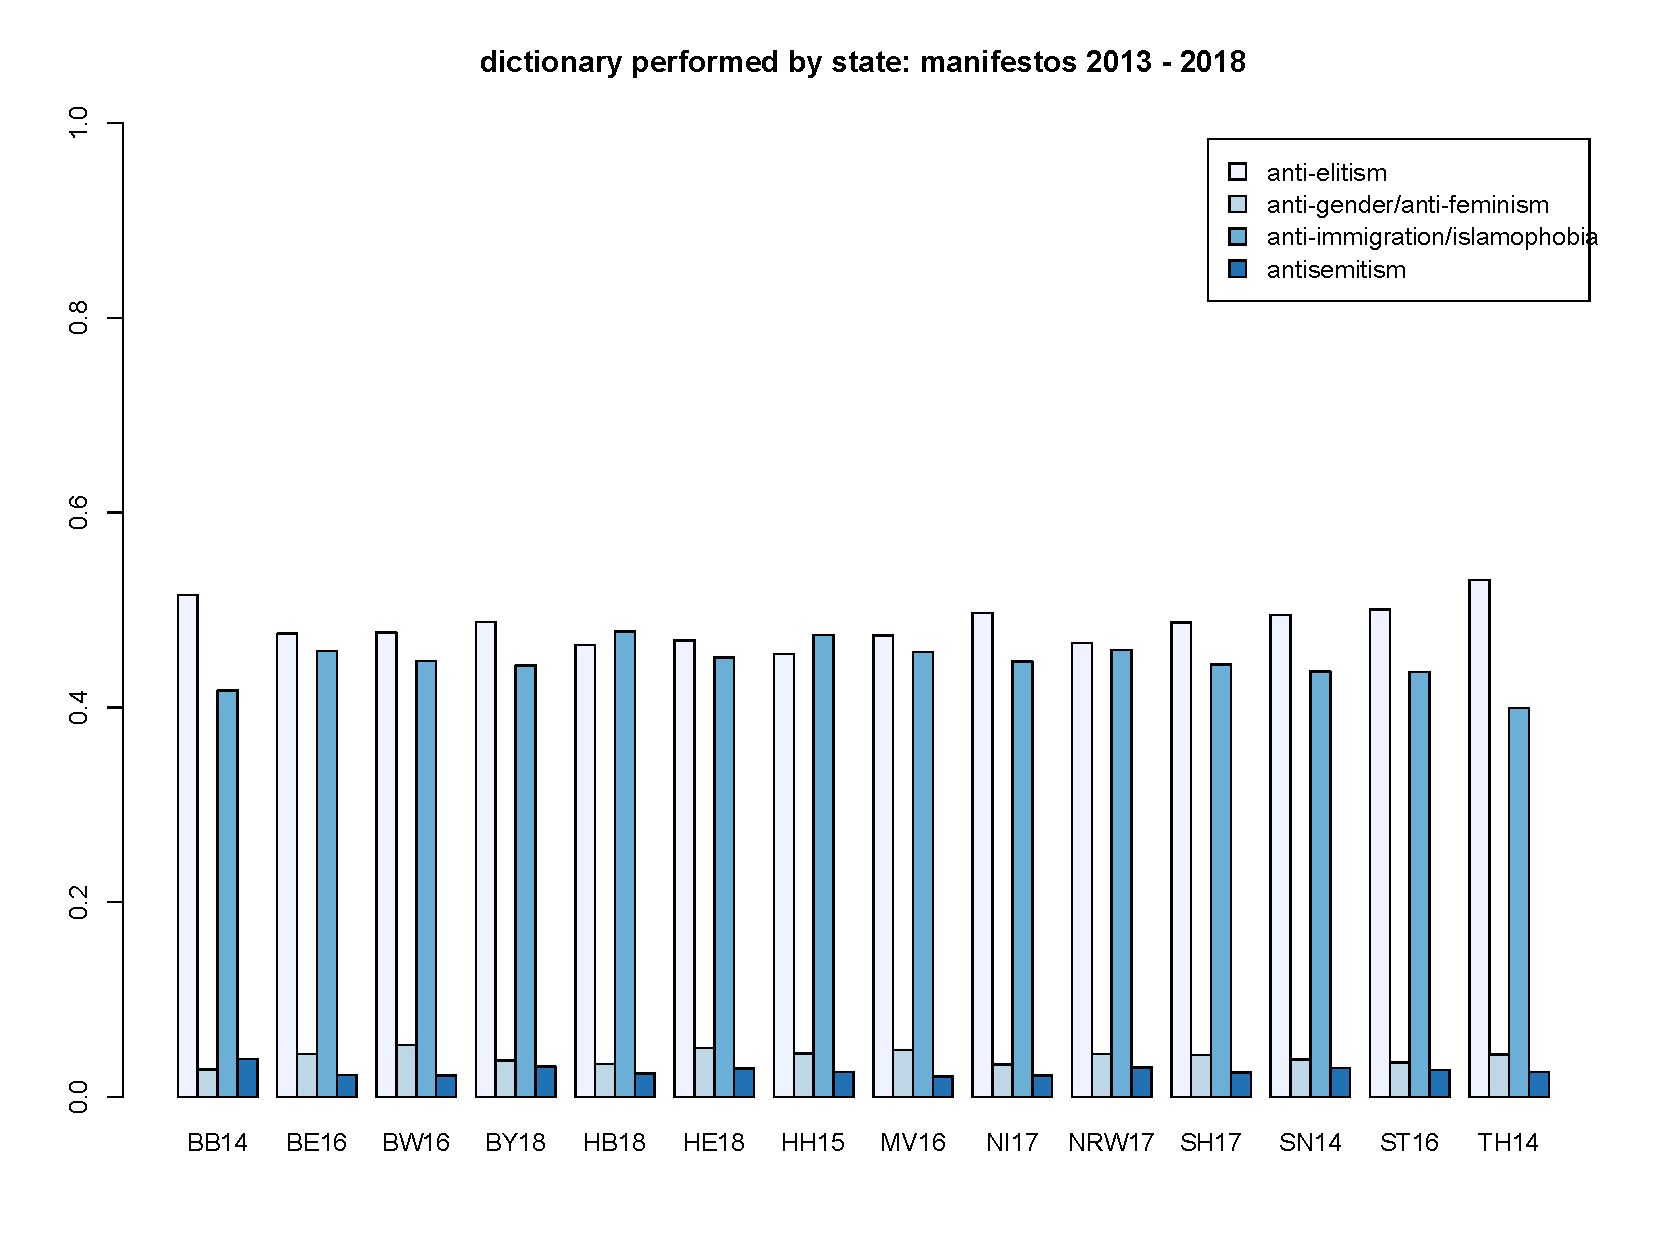
\includegraphics[width=\textwidth]{manifestos_dict_states_2013.pdf}
    \caption{a nice plot}
\end{figure}
\begin{figure}
    \centering
    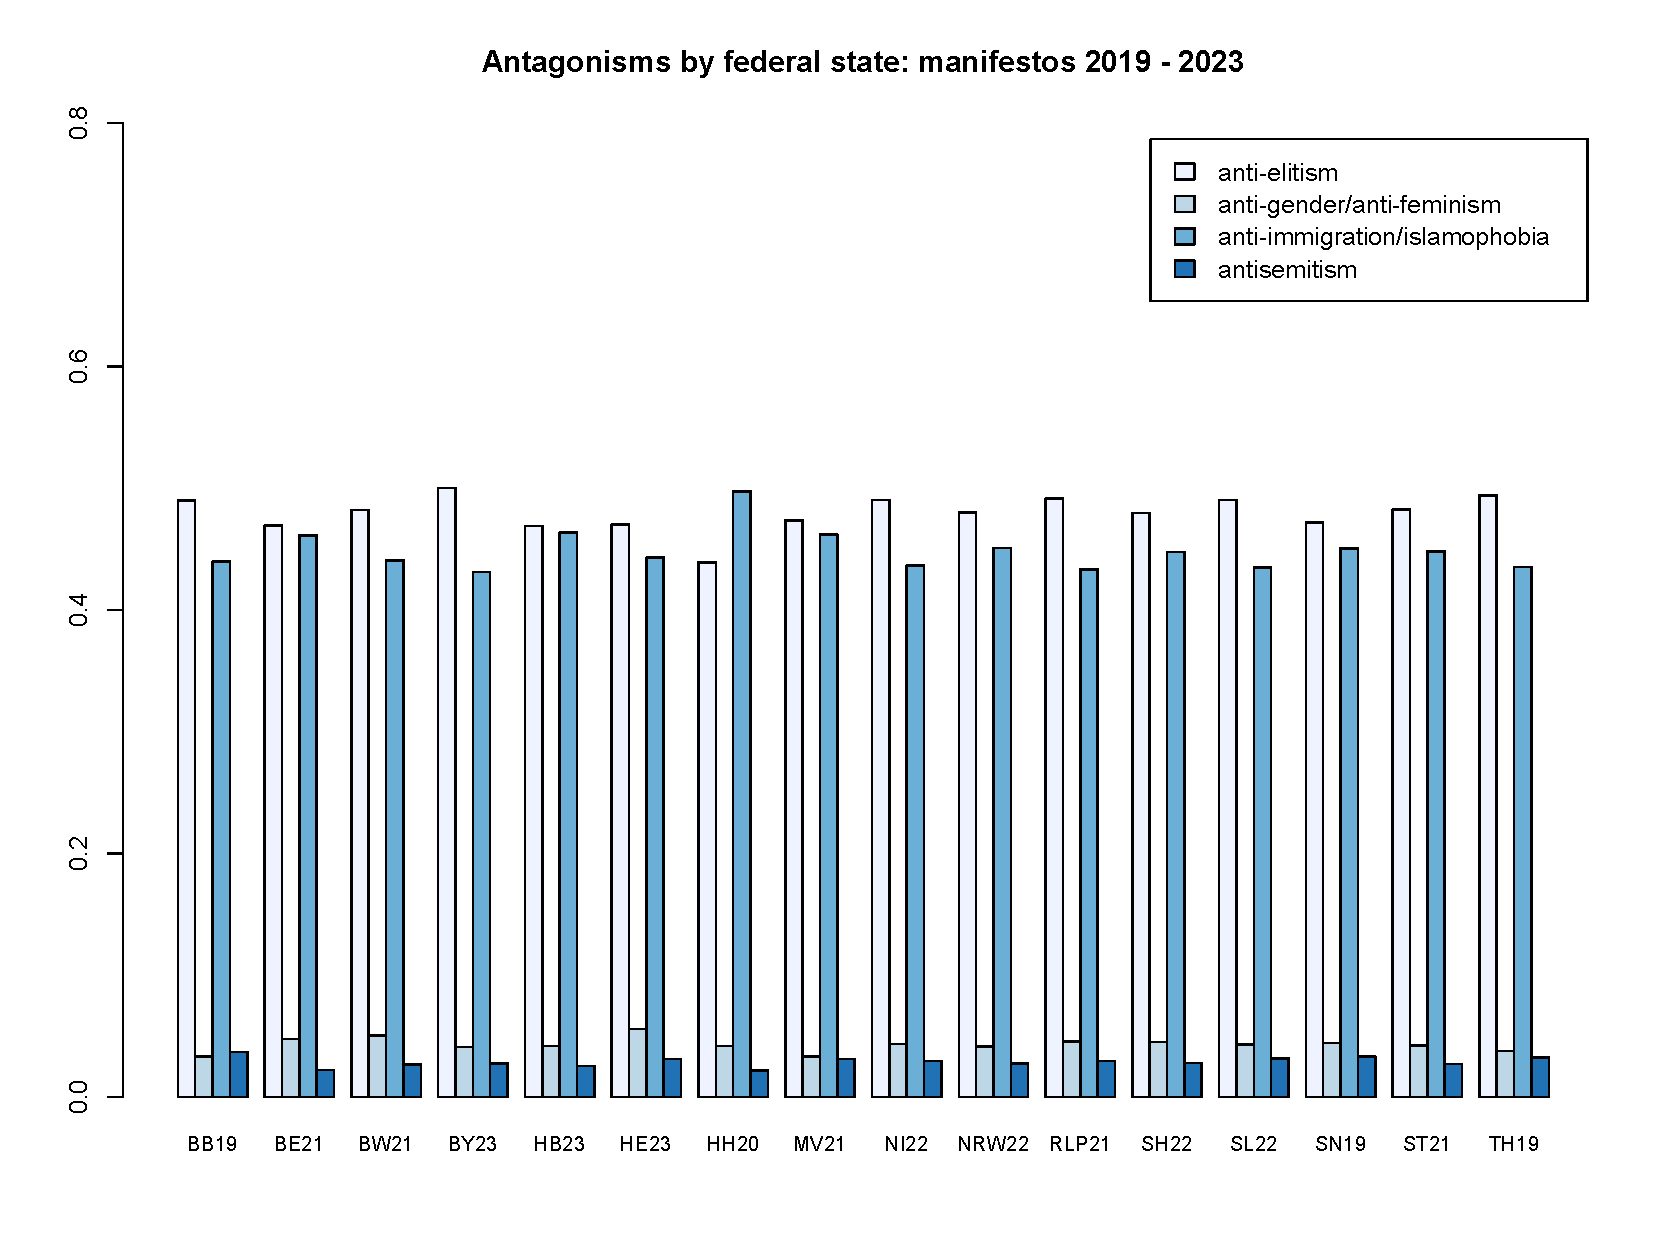
\includegraphics[width=\textwidth]{manifestos_dict_states_2018.pdf}
    \caption{a nice plot}
\end{figure}
\section{Temporal changes between East and West Germany}
\begin{figure}
    \centering
    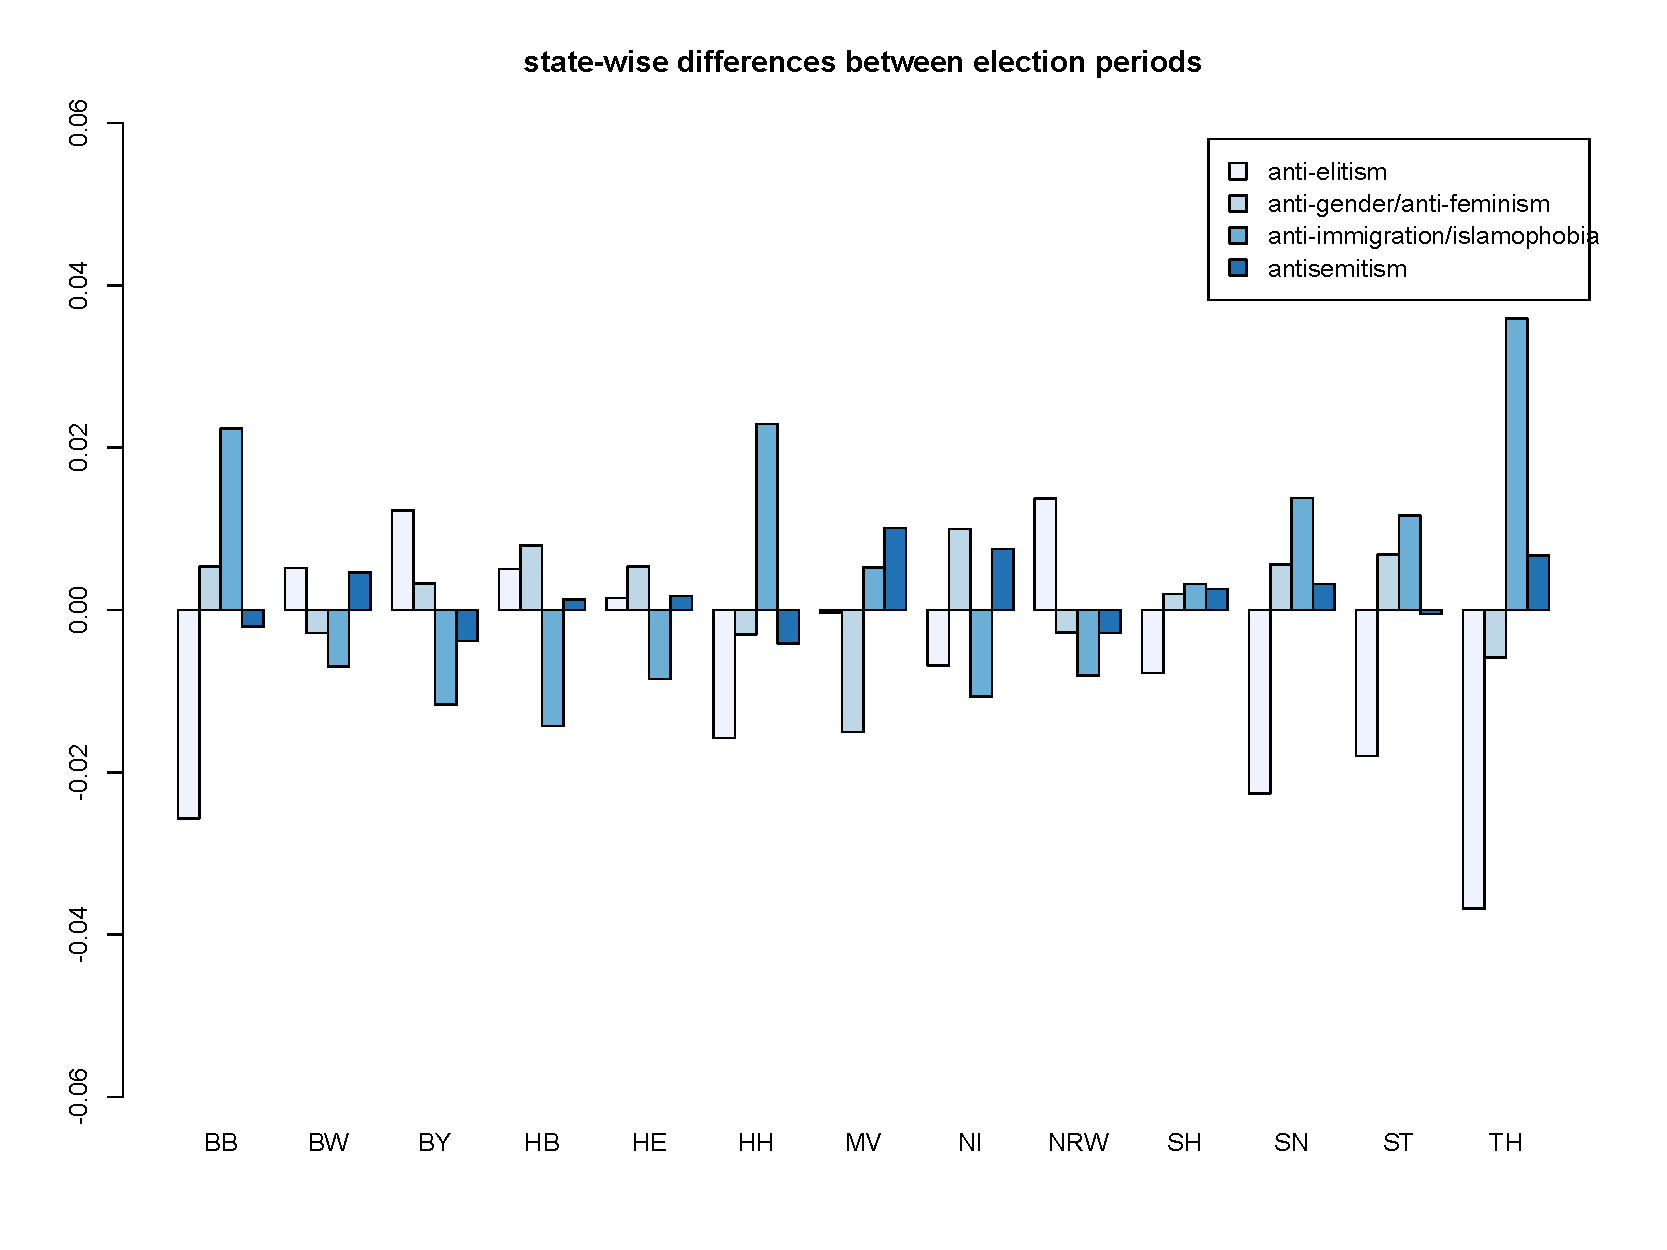
\includegraphics[width=\textwidth]{manifestos_dict_states_diffs.pdf}
    \caption{a nice plot}
\end{figure}
\begin{figure}
    \centering
    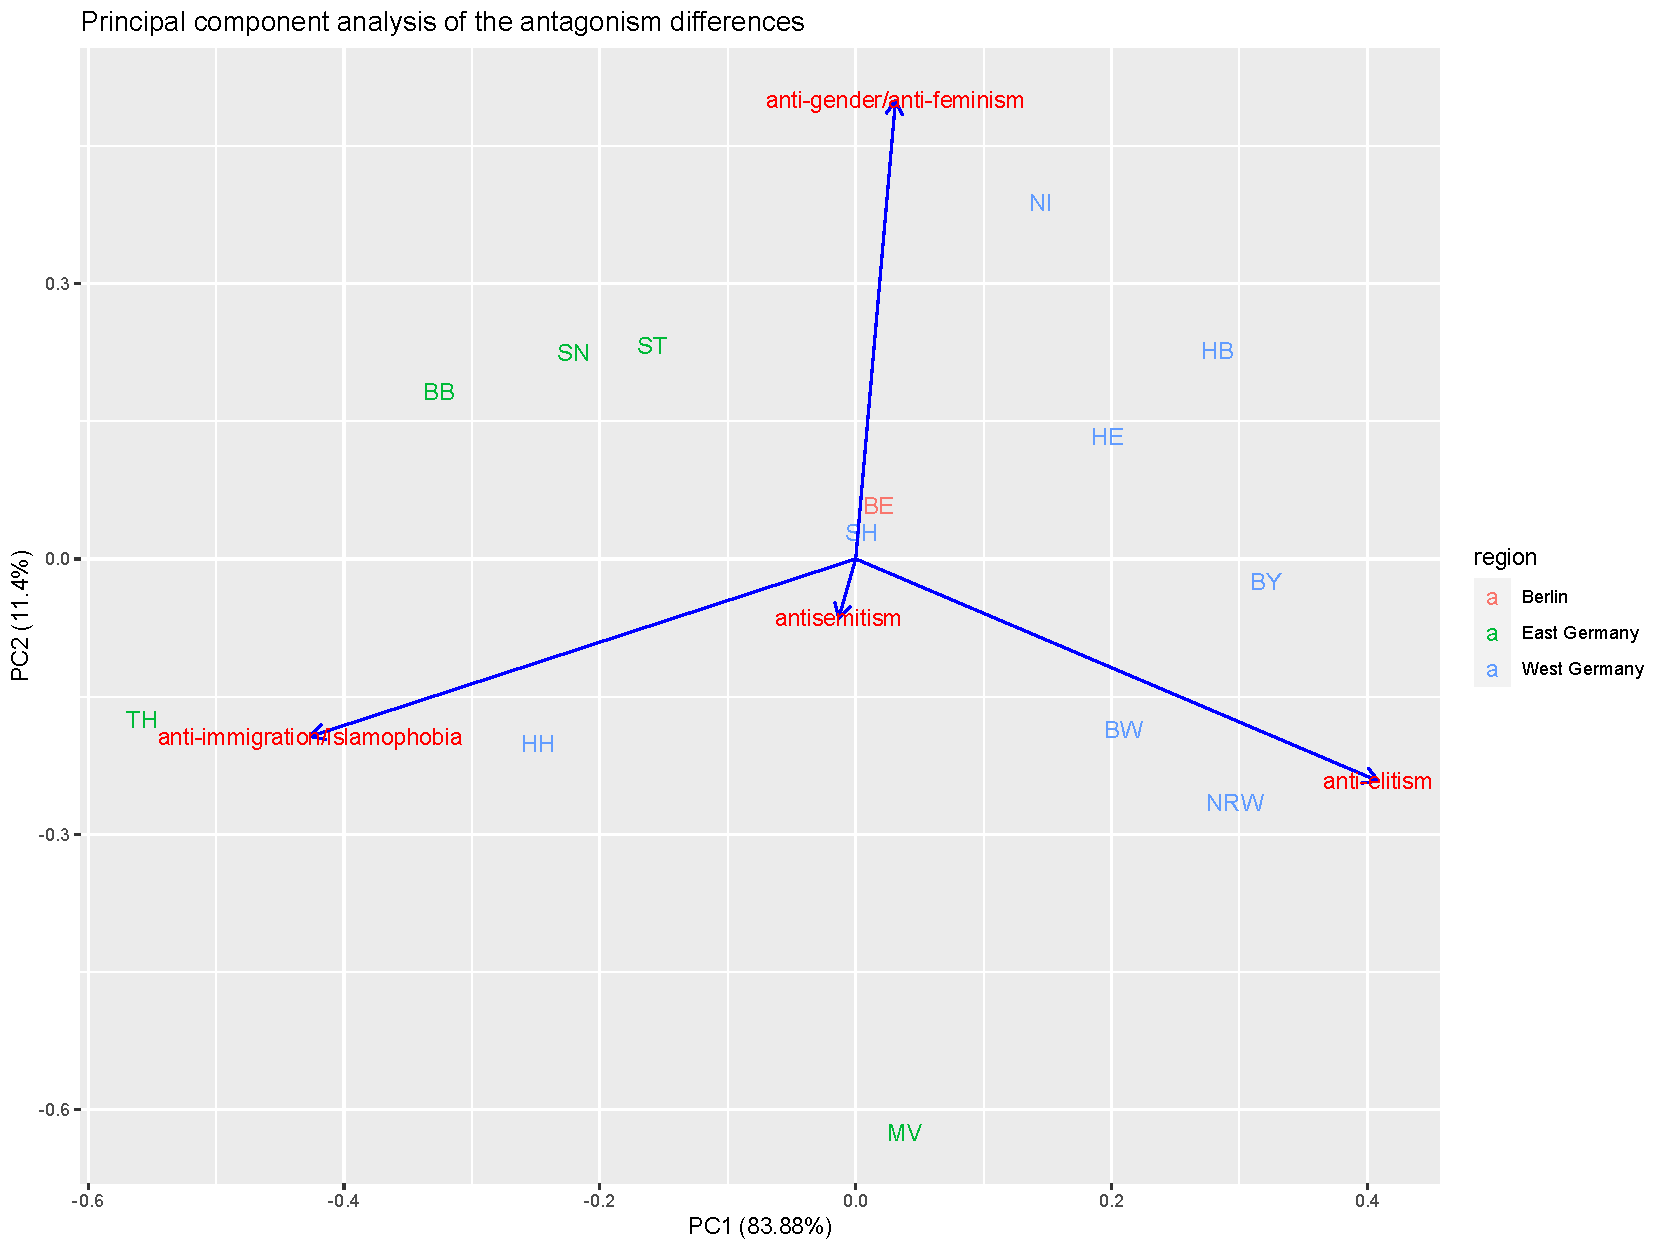
\includegraphics[width=\textwidth]{manifestos_diffs_pca.pdf}
    \caption{a nice plot}
\end{figure}
\begin{figure}
    \centering
    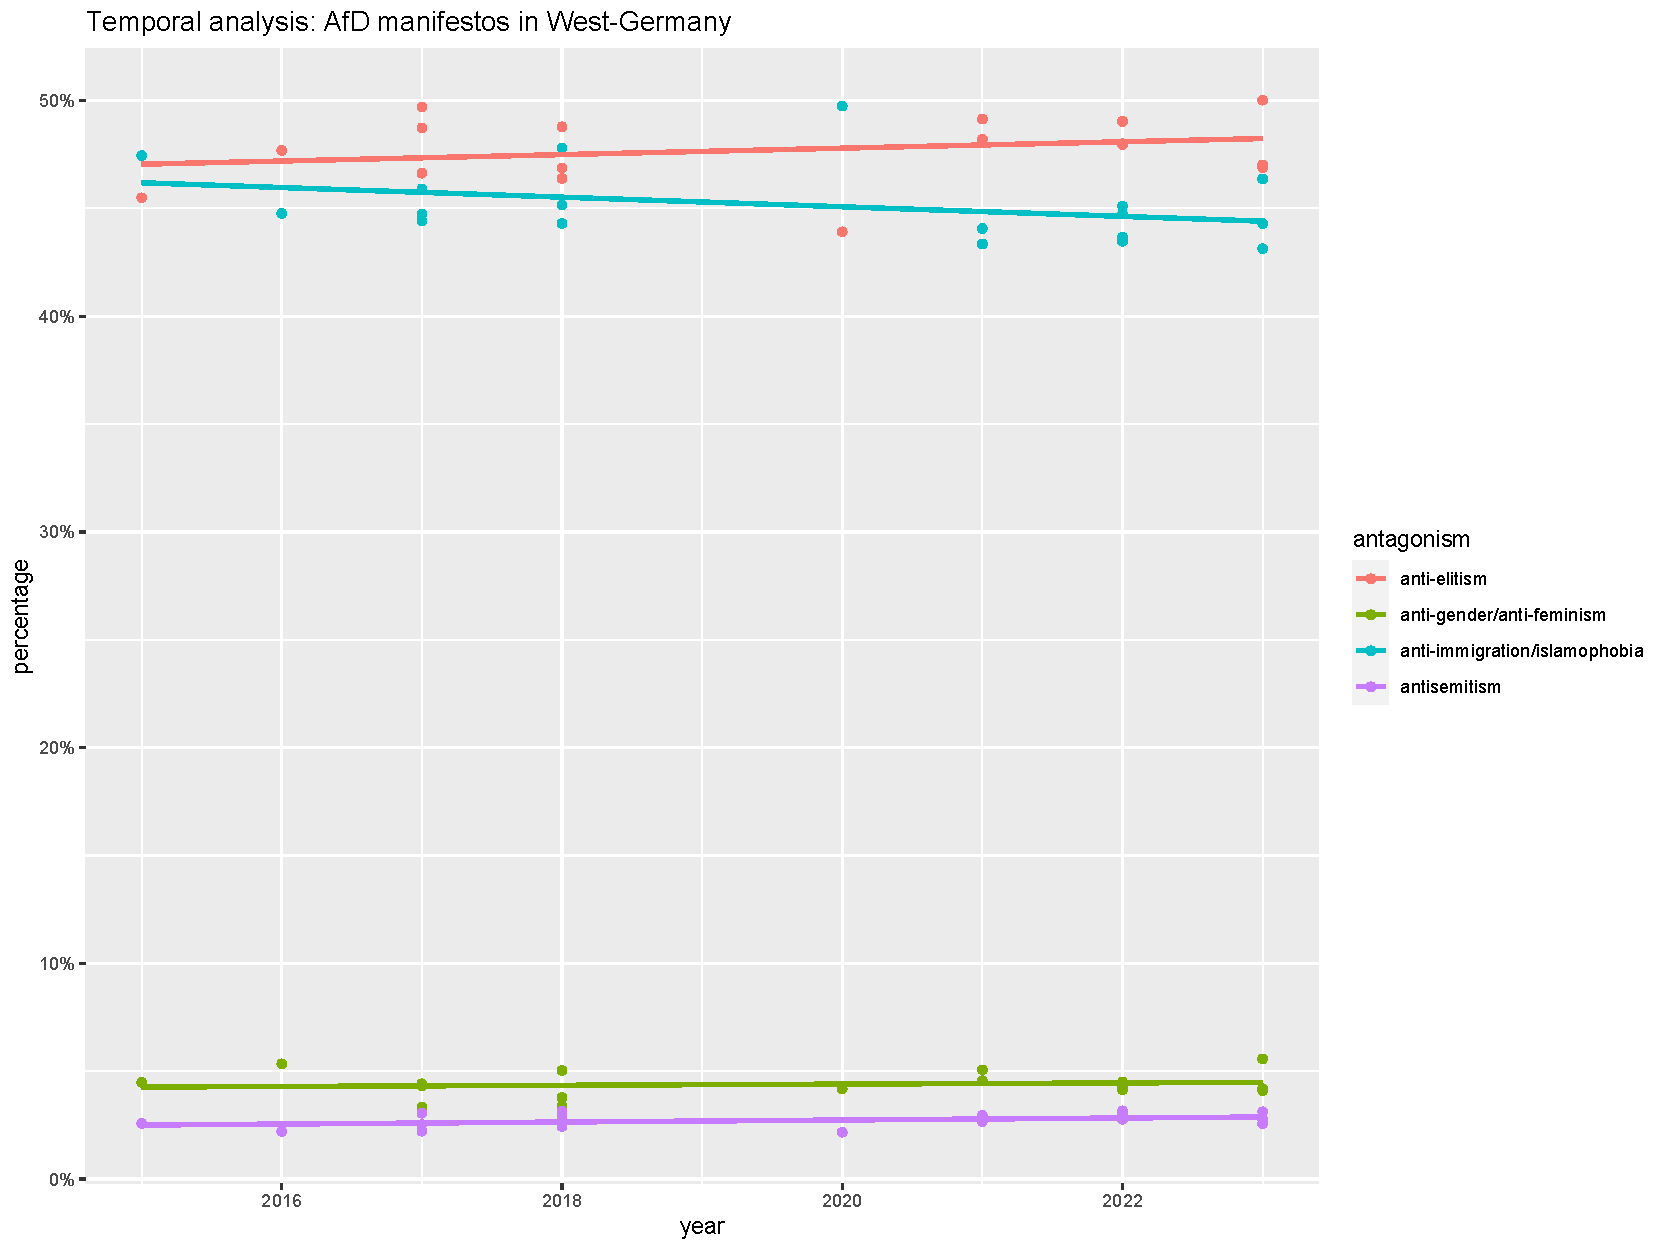
\includegraphics[width=\textwidth]{manifestos_temporal_regression_west.pdf}
    \caption{a nice plot}
\end{figure}
\begin{figure}
    \centering
    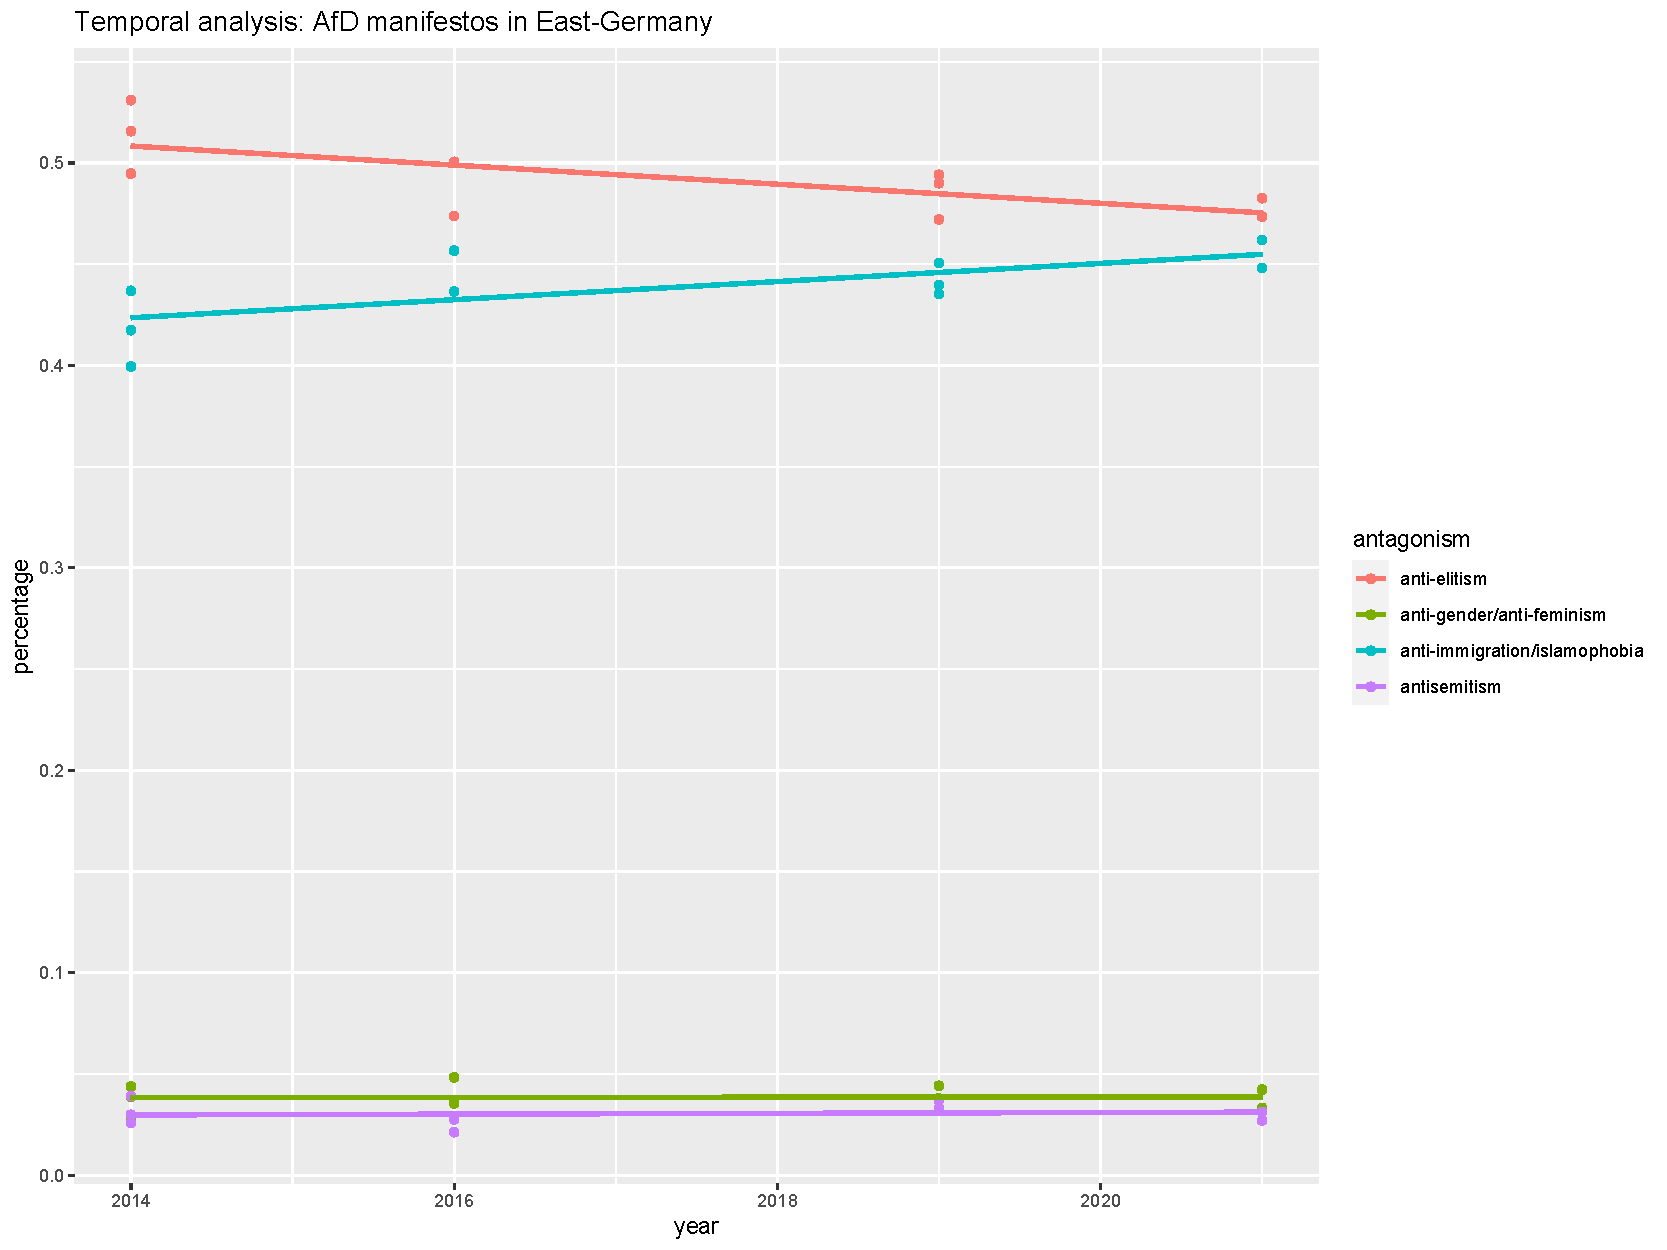
\includegraphics[width=\textwidth]{manifestos_temporal_regression_east.pdf}
    \caption{a nice plot}
\end{figure}
%%%%%
% 5 %
%%%%%
\chapter{Evaluation of the findings and validation}
\begin{figure}
    \centering
    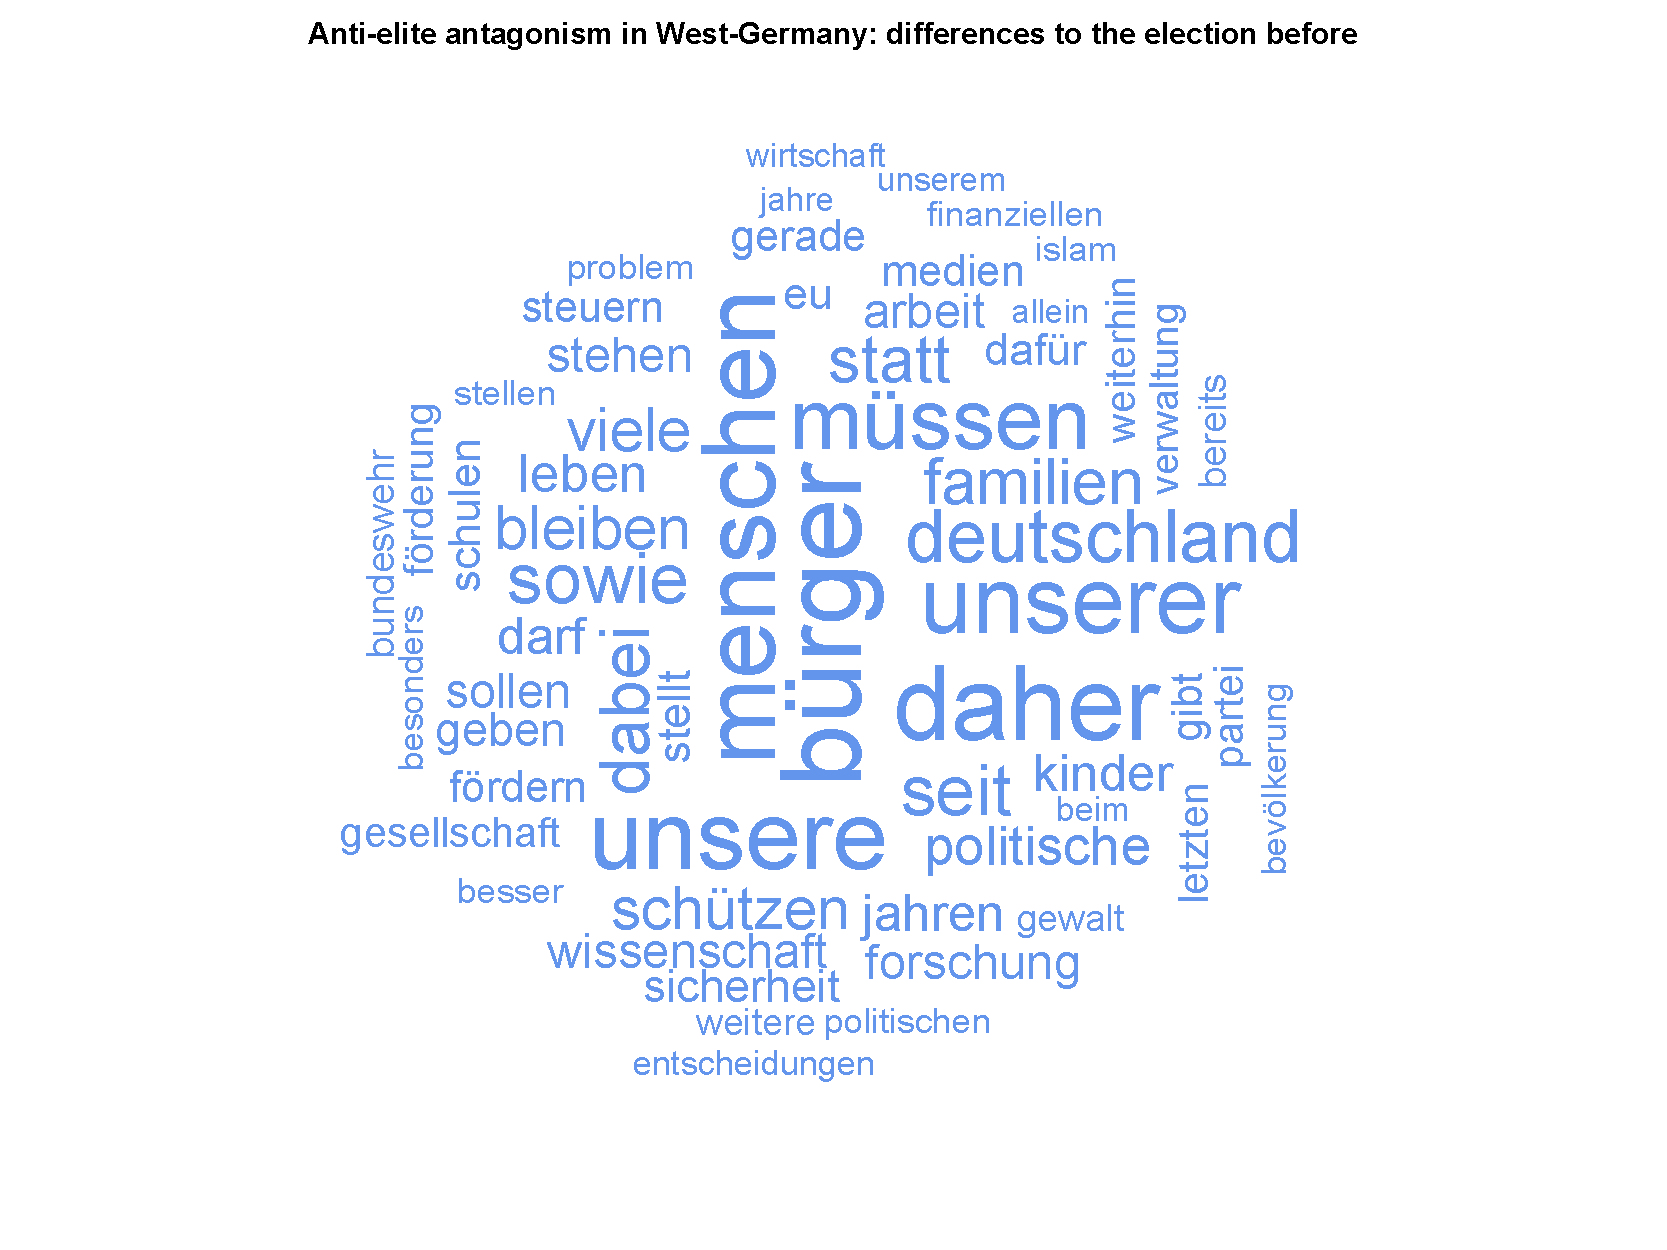
\includegraphics[width=0.9\textwidth]{manifestos_wordcloud_diffs_west.pdf}
    \caption{a nice plot}
\end{figure}
\begin{figure}
    \centering
    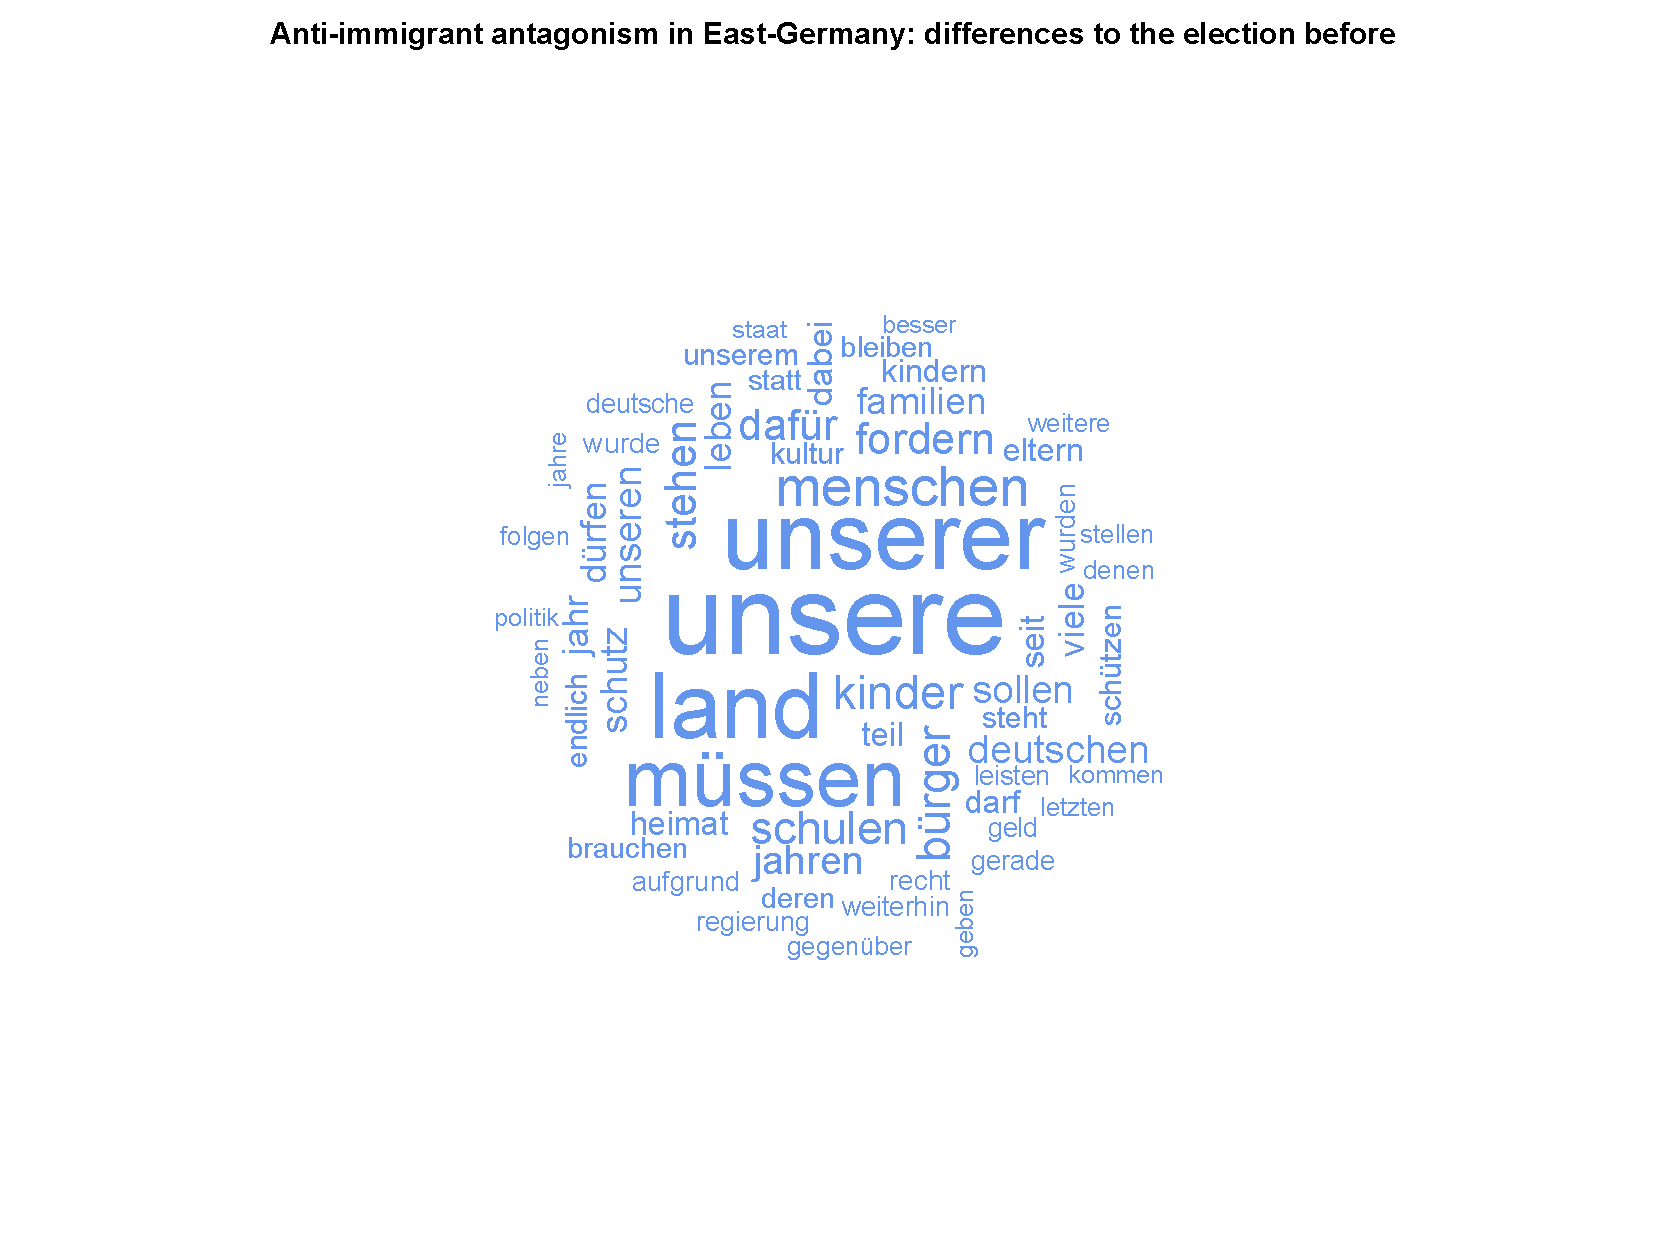
\includegraphics[width=0.9\textwidth]{manifestos_wordcloud_diffs_east.pdf}
    \caption{a nice plot}
\end{figure}
%%%%%
% 6 %
%%%%%
\chapter{Conclusion and final comments}

\bibliography{refs}

\end{document}